\documentclass[12pt]{report}
\usepackage{graphicx}
\usepackage{hyperref}
\usepackage{geometry}
\usepackage{enumitem}
\usepackage{booktabs}
\geometry{a4paper, margin=1in}

\begin{document}

\begin{center}

\includegraphics[width=2cm]{pes_logo.png} \\[0.5cm]
\textbf{\Large Dissertation on}\\[1cm]
\textbf{\Huge ``ICU Multi-Agent Synthetic Patient Data Generation Pipeline''}\\[1cm]

Submitted in partial fulfilment of the requirements for the award of degree of\\[1cm]
\textbf{\Large Master of Technology in}\\[1cm]
\textbf{\Large Data Seience \& AI}\\[1cm]

\textbf{Submitted by:}\\
\textbf{Surya Prtap Singh Shekhawat}\\
\textbf{PES2PGE24DS117}\\[1cm]

Under the guidance of\\
Dr/Prof. XXX\\
Prof. CSE, PES University\\[1cm]

January - May 20XX\\[1cm]

DEPARTMENT OF COMPUTER SCIENCE AND ENGINEERING\\
FACULTY OF ENGINEERING\\
PES UNIVERSITY\\[1cm]
(Established under Karnataka Act No. 16 of 2013)\\
Electronic City, Hosur Road, Bengaluru – 560 100, Karnataka, India
\end{center}

\newpage

\section*{Certificate}

This is to certify that the dissertation entitled ``ICU Multi-Agent Synthetic Patient Data Generation Pipeline'' is a bonafide work carried out by \textbf{Student Name (PES2PGXXCSXXX)} in partial fulfilment for the completion of Fourth Semester Project Phase - 2 (UE19CS651) in the Program of Study - Master of Technology in Computer Science and Engineering under the rules and regulations of PES University, Bengaluru during the period Jan. 20XX – May. 20XX.

\vspace{2cm}

\begin{flushright}
Dr. Guide Name\\
Prof. CSE
\end{flushright}

\newpage

\section*{Declaration}

We hereby declare that the Project Phase - 2 entitled ``ICU Multi-Agent Synthetic Patient Data Generation Pipeline'' has been carried out under the guidance of Dr. Guide Name, Department of CSE, and submitted in partial fulfilment of the course requirements for the award of the degree of Master of Technology in Computer Science and Engineering of PES University, Bengaluru during the academic semester January – May 2021.

\newpage

\section*{Acknowledgement}

I would like to express my gratitude to Dr. Guide Name, Department of Computer Science and Engineering, PES University, for her continuous guidance and support. I am also thankful to the project coordinators for their help throughout the process. I take this opportunity to thank the Chairperson of the Department of CSE, PES University, for the support and guidance. I am grateful to Dr. B.K. Keshavan, Dean of Faculty, and the university leadership for the opportunities provided. Finally, I extend heartfelt thanks to my family and friends for their constant support.

\newpage

\section*{Abstract}

Intensive Care Unit (ICU) research and machine-learning prototyping often require realistic patient trajectories, yet access to protected health information is restricted. This project implements an \texttt{icu\_agents} pipeline that generates synthetic ICU patient bundles using a multi-agent architecture. Specialized agents produce domain-specific outputs---hourly vitals, laboratory panels, radiology impressions, respiratory support parameters, rule-based risk scores, and clinician-style narrative summaries---orchestrated by a central \texttt{PatientPipeline} class. Patient identity and clinical context are modeled with Pydantic (\texttt{PatientState}), while diagnosis-conditioned clinical rules drive plausible data for conditions such as Sepsis, ARDS, Pneumonia, Aortic Dissection, COPD Exacerbation, and Heart Failure.

The system is exposed through a command-line entry point (\texttt{app.py}), a Streamlit dashboard for interactive generation, and two Apache Airflow DAGs: \texttt{icu\_multi\_agent\_pipeline} (sequential multi-task workflow with JSON/report/dashboard artifacts) and \texttt{icu\_temporal\_reasoning\_pipeline} (hourly severity tracing with branching on hypoxia and septic-shock thresholds and a coordinator agent for escalation recommendations). Outputs are persisted under \texttt{output/json}, \texttt{output/reports}, and \texttt{output/timelines}. The implementation demonstrates how workflow orchestration, modular agents, and structured synthetic data can support ICU analytics prototyping without compromising patient privacy.

\newpage

\tableofcontents
\newpage
\listoffigures
\newpage
\listoftables
\newpage

\chapter{Introduction}

Critical care environments generate high-frequency, multimodal data: vital signs, laboratory results, imaging reports, ventilator settings, and risk assessments. Building and testing analytics pipelines on real ICU data is constrained by privacy regulations, data-access agreements, and institutional review requirements. Synthetic data generation offers a practical alternative for pipeline development, agent orchestration experiments, and demonstration dashboards.

This project delivers the \texttt{icu\_agents} module within the ICU-pipeline repository. The system simulates complete synthetic ICU encounters by decomposing generation into specialized software agents, each responsible for one clinical modality. A shared patient state object accumulates outputs as the pipeline executes. The same agent logic is reused across local execution, a Streamlit user interface, and scheduled Airflow workflows, ensuring consistency between interactive and batch modes.

\section{Problem Statement}

Researchers and engineers working on ICU decision-support systems need representative patient records that span vitals time series, labs, imaging text, ventilation parameters, and derived risk metrics. Manually fabricating such records is error-prone and does not scale. Monolithic random generators, meanwhile, fail to preserve clinical coherence across modalities (e.g., sepsis should elevate lactate and perturb heart rate). The problem addressed by this project is to design and implement a modular, diagnosis-aware synthetic ICU data pipeline with clear orchestration, reproducible artifacts, and optional temporal reasoning for escalation scenarios.

\section{Objectives}

The primary objectives of the project are:
\begin{itemize}[noitemsep]
    \item To design a multi-agent architecture where each agent owns one clinical data domain (vitals, labs, radiology, respiratory, risk, narrative).
    \item To define a structured \texttt{PatientState} schema using Pydantic for type-safe patient bundles.
    \item To implement diagnosis-conditioned clinical rules for six ICU admission diagnoses.
    \item To provide a \texttt{PatientPipeline} orchestrator that sequences agent execution and returns a complete patient record.
    \item To integrate Apache Airflow DAGs for batch generation, artifact storage, and dashboard updates.
    \item To implement a temporal reasoning pipeline with hourly severity classification and branching on hypoxia and sepsis thresholds.
    \item To expose the system via CLI (\texttt{app.py}) and Streamlit for interactive demonstration.
\end{itemize}

\section{Scope of the Project}

The scope includes the Python package under \texttt{icu\_agents/}, comprising agents, orchestrator, synthetic clinical rules, data models, UI, and Airflow DAGs. Synthetic generation uses rule-based and stochastic sampling (Gaussian and uniform random variables); the configured OpenAI model identifier in \texttt{config.py} is reserved for future LLM integration, and the temporal DAG includes a placeholder LangGraph handoff task. The system does not connect to live EHR systems, train deep learning models on real data, or provide clinical decision support for actual patients. Airflow deployment is documented for Docker and WSL2; native Windows execution is limited to the core app and Streamlit due to POSIX dependencies.

\section{Organization of the Report}

Chapter~1 introduces the problem, objectives, and scope. Chapter~2 surveys related work and positions the proposed multi-agent approach. Chapter~3 specifies hardware, software, and functional requirements. Chapter~4 describes methodology, architecture, and workflows. Chapter~5 details implementation modules and dependencies. Chapter~6 discusses results and evaluation considerations. Chapter~7 concludes and outlines future enhancements.

\newpage

\chapter{Literature Survey}

Healthcare analytics increasingly relies on synthetic and semi-synthetic data when real cohorts are unavailable. Prior work on ICU scoring (e.g., severity indices) and sepsis detection emphasizes temporal vitals and laboratory markers such as lactate. Workflow engines such as Apache Airflow are widely used for ETL and ML pipelines in industry. Multi-agent and agentic AI frameworks (including LangChain and LangGraph, listed in project dependencies) support decomposed reasoning tasks, though this project's agents are currently implemented as plain Python classes with explicit orchestration.

\section{Existing Systems}

Existing approaches to ICU data simulation include:
\begin{itemize}[noitemsep]
    \item \textbf{Statistical simulators} that sample marginals independently, often breaking cross-field clinical consistency.
    \item \textbf{EHR-based synthetic generators} (e.g., GAN or copula-based) that require source data and substantial training infrastructure.
    \item \textbf{Rule-based clinical engines} embedded in research simulators, which encode domain knowledge but may lack modular orchestration.
    \item \textbf{Workflow-orchestrated pipelines} in production ML platforms, which schedule tasks but may not model clinical agents explicitly.
\end{itemize}

\section{Limitations of Existing Systems}

Monolithic generators are difficult to extend when new modalities (e.g., radiology narratives) are required. Black-box deep generative models demand large datasets and offer limited interpretability for education and pipeline testing. Systems without orchestration layers complicate scheduling, artifact versioning, and audit trails. Few lightweight prototypes combine interactive UI, batch DAG execution, and temporal branching for escalation logic in a single codebase.

\section{Proposed Solution}

The proposed \texttt{icu\_agents} system addresses these gaps through:
\begin{enumerate}[noitemsep]
    \item \textbf{Specialized agents} (\texttt{VitalsAgent}, \texttt{LabAgent}, \texttt{RadiologyAgent}, \texttt{RespiratoryAgent}, \texttt{RiskAgent}, \texttt{NarrativeAgent}) with diagnosis-aware parameters.
    \item \textbf{A unified \texttt{PatientState}} model aggregating all modalities.
    \item \textbf{\texttt{PatientPipeline}} for in-process orchestration and \textbf{Airflow DAGs} for production-style task graphs.
    \item \textbf{Temporal reasoning} with hourly severity labels and branch tasks for respiratory and sepsis escalation paths.
    \item \textbf{Persistent artifacts} (JSON bundles, text reports, timeline traces, dashboard snapshot).
\end{enumerate}

\newpage

\chapter{System Requirements Specification}

This chapter covers the system requirements, including hardware and software specifications necessary for the project.

\section{Hardware Requirements}

\begin{itemize}[noitemsep]
    \item 64-bit processor (Intel/AMD x64 or Apple Silicon with emulation).
    \item Minimum 8~GB RAM (16~GB recommended for Docker-based Airflow with PostgreSQL).
    \item 10~GB free disk space for Python environment, Docker images, and generated \texttt{output/} artifacts.
    \item Network access for initial dependency installation (pip, Docker image pulls).
\end{itemize}

\section{Software Requirements}

\begin{itemize}[noitemsep]
    \item \textbf{Operating system:} Windows 10/11 (app and Streamlit), WSL2 Ubuntu, or Linux/macOS for full Airflow support.
    \item \textbf{Python:} 3.10+ with \texttt{venv}.
    \item \textbf{Core libraries:} Pydantic, Pandas, NumPy, Faker, Streamlit, Matplotlib, scikit-learn, NetworkX (see \texttt{requirements.txt}).
    \item \textbf{Orchestration (optional):} Apache Airflow 2.x via Docker Compose (PostgreSQL 15 backend) or WSL2-native install.
    \item \textbf{Container runtime:} Docker Desktop (recommended for Airflow on Windows).
    \item \textbf{Version control:} Git.
\end{itemize}

\section{Functional Requirements}

\begin{enumerate}[noitemsep]
    \item \textbf{FR1:} Generate a synthetic patient with UUID, age, gender, and one of six ICU diagnoses.
    \item \textbf{FR2:} Produce 24-hour vital sign time series (heart rate, temperature, SpO$_2$, respiratory rate, systolic BP) with diagnosis-specific baselines.
    \item \textbf{FR3:} Generate laboratory results (WBC, lactate, creatinine, platelets, hemoglobin).
    \item \textbf{FR4:} Attach radiology report text mapped to diagnosis.
    \item \textbf{FR5:} Set respiratory support fields (mechanical ventilation flag, FiO$_2$, PEEP).
    \item \textbf{FR6:} Compute mortality, sepsis, and ICU deterioration risk scores from latest vitals and labs.
    \item \textbf{FR7:} Render a human-readable ICU narrative summary.
    \item \textbf{FR8:} Persist patient bundles and reports via Airflow tasks to \texttt{output/json} and \texttt{output/reports}.
    \item \textbf{FR9:} Update \texttt{latest\_dashboard.json} with key metrics after batch runs.
    \item \textbf{FR10:} Execute temporal pipeline with hourly severity trace, hypoxia/sepsis branching, and coordinator recommendations.
    \item \textbf{FR11:} Provide Streamlit UI to trigger generation and display narrative, vitals, labs, and risk JSON.
\end{enumerate}

\section{Non-Functional Requirements}

\begin{itemize}[noitemsep]
    \item \textbf{Modularity:} Each agent resides in a separate module under \texttt{agents/}.
    \item \textbf{Reproducibility:} Configurable random seed (\texttt{SEED = 42} in \texttt{config.py}) for future deterministic runs.
    \item \textbf{Extensibility:} New diagnoses can be added to \texttt{clinical\_rules.DIAGNOSES} and agent conditional logic.
    \item \textbf{Portability:} Docker Compose standardizes Airflow deployment across machines.
    \item \textbf{Usability:} Streamlit offers one-click patient generation for demonstrations.
    \item \textbf{Maintainability:} Pydantic models validate patient structure; Airflow task boundaries mirror agent boundaries.
\end{itemize}

\section{Use Case Diagram}
%\begin{figure}[h]
%\centering
%\includegraphics[width=0.8\textwidth]{use_case_diagram.png}
%\caption{Use Case Diagram}
%\end{figure}

Primary actors and use cases include: \textbf{Researcher/Operator} $\rightarrow$ run \texttt{app.py}, trigger Streamlit generation, or start Airflow DAGs; \textbf{Scheduler} $\rightarrow$ daily execution of \texttt{icu\_multi\_agent\_pipeline} and \texttt{icu\_temporal\_reasoning\_pipeline}; \textbf{System} $\rightarrow$ write JSON/report/timeline artifacts and update dashboard metadata.

\newpage

\chapter{Proposed Methodology}

This chapter explains the overall methodology, system architecture, data flow, and algorithms used in the \texttt{icu\_agents} implementation.

\section{System Architecture}

The architecture has three layers:
\begin{enumerate}[noitemsep]
    \item \textbf{Presentation:} \texttt{app.py} (CLI) and \texttt{ui/streamlit\_app.py} (web UI).
    \item \textbf{Orchestration:} \texttt{orchestrator/patient\_pipeline.py} for synchronous multi-agent execution; Apache Airflow DAGs for asynchronous task graphs.
    \item \textbf{Agent layer:} Six agents plus \texttt{synthetic/clinical\_rules.py} for base demographics and diagnosis selection.
\end{enumerate}

Data flows from \texttt{generate\_base\_patient()} into a \texttt{PatientState} instance. Agents populate vitals, labs, radiology, respiratory, and risk fields in sequence; \texttt{NarrativeAgent} consumes the complete state. Airflow DAGs replicate this flow as separate tasks passing a dictionary state, with additional storage and dashboard tasks.

\begin{figure}[h]
\centering
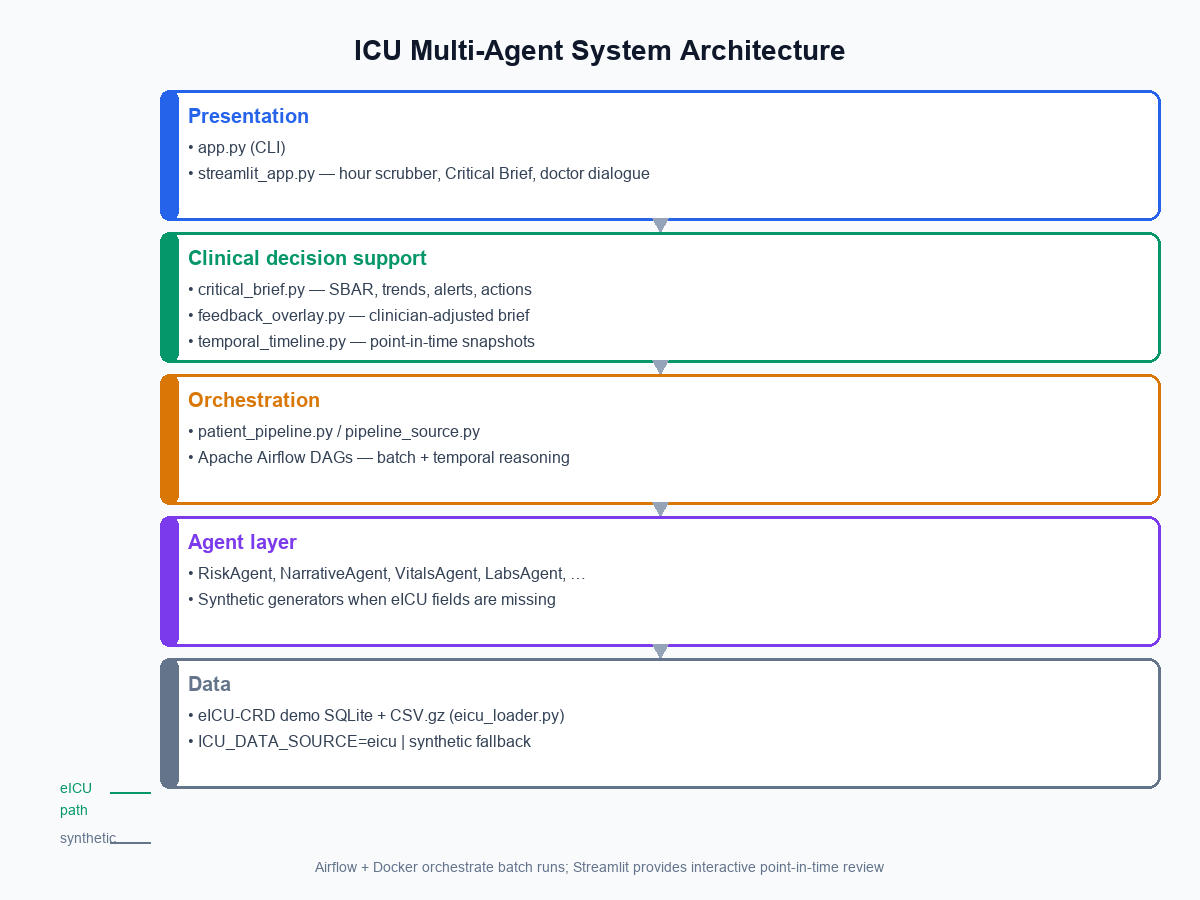
\includegraphics[width=0.8\textwidth]{system_architecture.png}
\caption{System Architecture Diagram (multi-agent orchestrator, agents, Airflow, and output stores)}
\end{figure}

\section{Algorithm or Model Description}

\textbf{Base patient generation.} \texttt{generate\_base\_patient()} randomly selects age (24--88), gender (Male/Female), and diagnosis from six conditions.

\textbf{VitalsAgent.} For each hour in a 24-hour window, samples vitals from Gaussian distributions centered on diagnosis-specific baselines (e.g., Sepsis: higher heart rate and temperature, lower SpO$_2$; ARDS: SpO$_2$ baseline 85\%).

\textbf{LabAgent.} Samples WBC, lactate, creatinine, platelets, and hemoglobin with diagnosis-adjusted means (elevated lactate and WBC for Sepsis).

\textbf{RadiologyAgent.} Returns a fixed impression string per diagnosis from a lookup table.

\textbf{RespiratoryAgent.} Sets mechanical ventilation and FiO$_2$/PEEP ranges for ARDS and Sepsis; otherwise room-air defaults.

\textbf{RiskAgent.} Rule-based scoring: adds weighted points if SpO$_2$ $<$ 90, heart rate $>$ 120, lactate $>$ 4, or creatinine $>$ 2; caps mortality risk at 100 and derives correlated sepsis and deterioration scores.

\textbf{Temporal reasoning (Airflow).} \texttt{build\_hourly\_reasoning\_trace} labels each hour as \textit{stable}, \textit{worsening}, or \textit{critical} from SpO$_2$ and heart-rate thresholds. Branch operators route to escalation tasks when SpO$_2$ $<$ 85 or lactate $>$ 4. \texttt{coordinator\_agent} merges paths and recommends FiO$_2$/PEEP adjustments or sepsis actions.

\section{Workflow Diagram}

\textbf{Local pipeline (\texttt{PatientPipeline.run}):}
\begin{enumerate}[noitemsep]
    \item Generate base patient $\rightarrow$ create \texttt{PatientState} with UUID.
    \item VitalsAgent $\rightarrow$ LabAgent $\rightarrow$ RadiologyAgent $\rightarrow$ RespiratoryAgent.
    \item RiskAgent $\rightarrow$ NarrativeAgent $\rightarrow$ return patient.
\end{enumerate}

\textbf{Airflow \texttt{icu\_multi\_agent\_pipeline}:}
\texttt{generate\_patient} $\rightarrow$ \texttt{generate\_vitals} $\rightarrow$ \texttt{generate\_labs} $\rightarrow$ \texttt{generate\_radiology} $\rightarrow$ \texttt{generate\_respiratory} $\rightarrow$ \texttt{calculate\_risk} $\rightarrow$ \texttt{generate\_narrative} $\rightarrow$ \texttt{store\_patient\_bundle} $\rightarrow$ \texttt{update\_dashboard}.

\textbf{Airflow \texttt{icu\_temporal\_reasoning\_pipeline}:}
\texttt{generate\_temporal\_bundle} $\rightarrow$ \texttt{build\_hourly\_reasoning\_trace} $\rightarrow$ parallel branch tasks (hypoxia, sepsis) $\rightarrow$ \texttt{coordinator\_agent} $\rightarrow$ \texttt{optional\_langgraph\_handoff} $\rightarrow$ \texttt{generate\_temporal\_narrative} $\rightarrow$ \texttt{store\_temporal\_outputs}.

\newpage

\chapter{Implementation Details}

This chapter provides details of the development process, programming languages used, tools and libraries, module layout, and evaluation approach.

\section{Development Environment}

Development was carried out in Python using a virtual environment (\texttt{python -m venv .venv}). The package root is \texttt{icu\_agents/}. Local execution:
\begin{verbatim}
cd icu_agents
pip install -r requirements.txt
python app.py
streamlit run ui/streamlit_app.py
\end{verbatim}
Airflow is deployed via \texttt{docker-compose.yml} (PostgreSQL, webserver on port 8080, scheduler) with DAGs mounted from \texttt{airflow/dags/}. Project configuration in \texttt{config.py} defines \texttt{OPENAI\_MODEL}, \texttt{MAX\_ICU\_HOURS = 72}, and \texttt{SEED = 42}.

\section{Dataset Description}

The system does not consume an external labeled dataset. Synthetic records are generated on demand. Each patient bundle includes:
\begin{itemize}[noitemsep]
    \item Demographics: \texttt{patient\_id}, \texttt{age}, \texttt{gender}, \texttt{diagnosis}.
    \item \texttt{vitals}: list of 24 hourly dictionaries (timestamp, heart\_rate, temperature, spo2, resp\_rate, systolic\_bp).
    \item \texttt{labs}: WBC, Lactate, Creatinine, Platelets, Hemoglobin.
    \item \texttt{radiology}: report text; \texttt{respiratory}: ventilation parameters.
    \item \texttt{risk\_scores}: mortality\_risk, sepsis\_risk, icu\_deterioration\_risk.
    \item \texttt{narrative}: formatted clinical summary string.
\end{itemize}
Temporal runs add \texttt{reasoning\_trace}, escalation blocks, and \texttt{temporal\_narrative}. Artifacts are written to \texttt{output/json}, \texttt{output/reports}, and \texttt{output/timelines}.

\section{Model Implementation}

Key modules and responsibilities:

\begin{table}[h]
\centering
\begin{tabular}{@{}ll@{}}
\toprule
\textbf{Module} & \textbf{Role} \\
\midrule
\texttt{models/patient\_state.py} & Pydantic \texttt{PatientState} schema \\
\texttt{synthetic/clinical\_rules.py} & Diagnosis list and base patient sampling \\
\texttt{agents/vitals\_agent.py} & Hourly vitals time series \\
\texttt{agents/lab\_agent.py} & Laboratory panel generation \\
\texttt{agents/radiology\_agent.py} & Imaging report lookup \\
\texttt{agents/respiratory\_agent.py} & Ventilation settings \\
\texttt{agents/risk\_agent.py} & Rule-based risk scoring \\
\texttt{agents/narrative\_agent.py} & Textual ICU summary \\
\texttt{orchestrator/patient\_pipeline.py} & Agent sequencing \\
\texttt{airflow/dags/icu\_multi\_agent\_pipeline.py} & Batch multi-agent DAG \\
\texttt{airflow/dags/icu\_temporal\_reasoning\_pipeline.py} & Temporal branching DAG \\
\texttt{ui/streamlit\_app.py} & Interactive UI \\
\bottomrule
\end{tabular}
\caption{Implementation module map}
\end{table}

\section{Evaluation Metrics}

Because outputs are synthetic, evaluation focuses on pipeline correctness and clinical plausibility rather than predictive accuracy against gold labels:
\begin{itemize}[noitemsep]
    \item \textbf{Structural validity:} JSON bundles conform to expected keys; Pydantic validation on \texttt{PatientState}.
    \item \textbf{Diagnosis consistency:} Sepsis cases exhibit elevated lactate/WBC and appropriate radiology strings.
    \item \textbf{Risk monotonicity:} Higher lactate and lower SpO$_2$ increase mortality risk scores.
    \item \textbf{Temporal severity:} Critical hours in reasoning trace align with threshold breaches.
    \item \textbf{Operational metrics:} DAG success rate, artifact creation under \texttt{output/}, dashboard update latency.
\end{itemize}
Future work may add distributional comparison to published ICU statistics and LLM-judged narrative quality.

\newpage

\chapter{Results and Discussion}

The pipeline was exercised through CLI runs, Streamlit sessions, and repeated Airflow DAG triggers. Each successful run produces a unique \texttt{patient\_id} and persisted artifacts.

\section{Result Analysis}

\textbf{Single-patient generation.} Running \texttt{python app.py} prints the full \texttt{model\_dump()} JSON and the narrative block, confirming end-to-end agent integration.

\textbf{Multi-agent Airflow DAG.} The \texttt{icu\_multi\_agent\_pipeline} writes \texttt{\{patient\_id\}.json} and \texttt{\{patient\_id\}.txt} under \texttt{output/}, and refreshes \texttt{latest\_dashboard.json} with diagnosis, mortality risk, latest SpO$_2$, and paths to artifacts.

\textbf{Temporal reasoning DAG.} The \texttt{icu\_temporal\_reasoning\_pipeline} stores \texttt{\{patient\_id\}\_temporal\_trace.json} and \texttt{\{patient\_id\}\_temporal\_report.txt}. Branching correctly selects respiratory escalation when terminal SpO$_2$ falls below 85\% and sepsis escalation when lactate exceeds 4~mmol/L. The coordinator merges recommendations (FiO$_2$/PEEP bumps, sepsis action list) into the final bundle.

\textbf{Streamlit UI.} Operators can generate patients on demand and inspect narrative, vitals JSON, labs JSON, and risk scores without using the terminal.

\textbf{Discussion.} The rule-based approach yields interpretable, fast generation suitable for pipeline testing. Stochastic sampling introduces variability across runs while preserving diagnosis-specific tendencies. Limitations include simplified risk scoring (not calibrated to APACHE/SOFA), static radiology templates, and placeholder LangGraph integration. The architecture nonetheless demonstrates clear separation of concerns and straightforward extension points for ML-based agents.

%\begin{figure}[h]
%\centering
%\includegraphics[width=0.8\textwidth]{results_graph.png}
%\caption{Model Performance Graph}
%\end{figure}

\newpage

\chapter{Conclusion and Future Work}

\section{Conclusion}

This project implemented the \texttt{icu\_agents} multi-agent synthetic ICU patient data generation pipeline. Six specialized agents, a Pydantic patient model, and a central orchestrator produce coherent multimodal records for six critical-care diagnoses. Apache Airflow extends the design with schedulable DAGs, artifact persistence, dashboard metadata, and a temporal reasoning workflow with clinical branching. CLI and Streamlit interfaces make the system accessible for local demonstration. The work shows that modular agents combined with workflow orchestration can support privacy-preserving ICU analytics prototyping.

\section{Future Work}

\begin{itemize}[noitemsep]
    \item Integrate LLM-based agents using \texttt{OPENAI\_MODEL} and LangGraph for stateful reasoning (\texttt{optional\_langgraph\_handoff} task stub).
    \item Calibrate risk scores against established ICU severity scores (SOFA, APACHE).
    \item Expand diagnoses, medications, fluid balance, and nursing notes.
    \item Add unit tests and validation suites comparing synthetic distributions to published ICU benchmarks.
    \item Enable deterministic replay via centralized random seeding across all agents.
    \item Connect outputs to downstream ML training pipelines and FHIR-compatible export formats.
    \item Deploy monitoring and data-quality checks on Airflow task failures and artifact schema drift.
\end{itemize}

\newpage

\begin{thebibliography}{99}

\bibitem{ref1} Johnson, A.E.W., et al., ``MIMIC-III, a freely accessible critical care database'', \textit{Scientific Data}, 2016.

\bibitem{ref2} Seymour, C.W., et al., ``Assessment of Clinical Criteria for Sepsis'', \textit{JAMA}, 2016.

\bibitem{ref3} Ranieri, V.M., et al., ``Acute Respiratory Distress Syndrome: The Berlin Definition'', \textit{JAMA}, 2012.

\bibitem{ref4} Vaswani, A., et al., ``Attention is All You Need'', \textit{Advances in Neural Information Processing Systems (NeurIPS)}, 2017.

\bibitem{ref5} Devlin, J., Chang, M.W., Lee, K., and Toutanova, K., ``BERT: Pre-training of Deep Bidirectional Transformers for Language Understanding'', \textit{arXiv preprint arXiv:1810.04805}, 2018.

\bibitem{ref6} Apache Software Foundation, ``Apache Airflow Documentation'', \url{https://airflow.apache.org/docs/}, 2024.

\bibitem{ref7} Chase, H., ``LangChain: Building applications with LLMs through composability'', \url{https://github.com/langchain-ai/langchain}, 2023.

\bibitem{ref8} Chollet, F., ``Deep Learning with Python'', Manning Publications, 2017.

\bibitem{ref9} Bishop, C.M., ``Pattern Recognition and Machine Learning'', Springer, 2006.

\bibitem{ref10} Beaulieu-Jones, B.K., et al., ``Privacy-preserving generative deep neural networks for synthetic patient data generation'', \textit{Network and Systems Medicine}, 2019.

% Add more references below as needed

\end{thebibliography}
\end{document}
